\documentclass{article}
\usepackage[utf8]{inputenc}
\usepackage[T1]{fontenc}
\usepackage{graphicx}
\usepackage{hyperref}
\usepackage{geometry}
\geometry{margin=1in}

\title{ESCHARA}
\date{Encyclopaedia Britannica (1771)}

\begin{document}
\maketitle

\section*{Historical source}
\textbf{Entry ID:} \texttt{entry-eschara-1473} \\
\textbf{Volume ID:} 149979622 \\
\textbf{Character Count:} 2406

\subsection*{Extracted Text}
ESCHARA, in natural history, the name of a fpec-
ence localizing, the the theories of which we in these
they are of a study or coral like hardwood, and reminds
a woven cloth in their texture; and the microtype ins-
forms us, that they confidif arrangements of very
small cells, whose furfaces appear much in this form, Linnmus makes it a species of millepora, in the clafs
oil hobphory. See Place CLXVII, fig. you.

The narrow-level borrowback, fig. to divides as it
rifes, into narrow leaves made up of regular rows of
obbing figures shaped into placed alternates by each
other, and opposed to an equal number on the other
file of the leaf, like an honeycomb, from their leaves
proved, other still familiar difference numifications,
many of which femen to be connected at the lower part
by tub), as in the corailings; by which means they
can play to and for those freely in the waters—Give
the natural appearance of this condition. E. reporters
two leaves with their shall and cells magnified. E. t
is a covid fiction of one of the leaves at E, flowing the
partition and inner form of their cells.

The broad-leaved brownwork, fig. to, when fresh
taken out of the tea, it of a spongy salt texture, and
finels very little, but when it has fun for time time
on the floor, it becomes iffi and honey, like forms fort
of nutrients below. Beff furthest, when examined by
glallies, appears to be covered with cells; and, when a
piece of it is cut across, one may discover the thin
numbers that there was a large to the cell of each face.

The form of the cells is very remarkable, each
one being needed at the top, and contracted a littered
the lower part of the files to make sure for the reaches
of the two next adjoining cells; fo that by this par-
ticulus contribution so soon is hold. The utterance
of the cells is immediately under the arch, each cell,
and the walls of the cells femen to be fortified with
ripises. Julfine different fossil polyps extending
themselves out of their cells, which lie has identified
in the memoirs of the Academy of Sciences 1742--
Gives the natural appearance is a leafy branch of
this condition.

At the entrance of many of the cells a small triflu-
cus body like a bivalve shell in discovered: E. z, the
figure of the cell, with the fluid in it; it is of a tranfi-
parent anber colours, do clear that one may feel the
dead until through its repetiended by the block-
fpot.



\section*{Source record}
\begin{itemize}
\item \textbf{Dataset:} \texttt{NationalLibraryOfScotland/encyclopaedia\_britannica\_illustrated}
\item \textbf{Dataset Revision:} \texttt{309f765b1ecc83e0a7f7762e44b4a927a7555443}
\item \textbf{Page ID:} \texttt{britannica:309f765b1ecc83e0a7f7762e44b4a927a7555443:train:1473} \\
  \textbf{Filename:} \texttt{page-1473-b3b602ef6a3d.jpg} \\
  \textbf{Row Index:} 1473 \\
  \textbf{SHA256:} \texttt{b3b602ef6a3d4961...}
\end{itemize}

\begin{figure}[h]
\centering
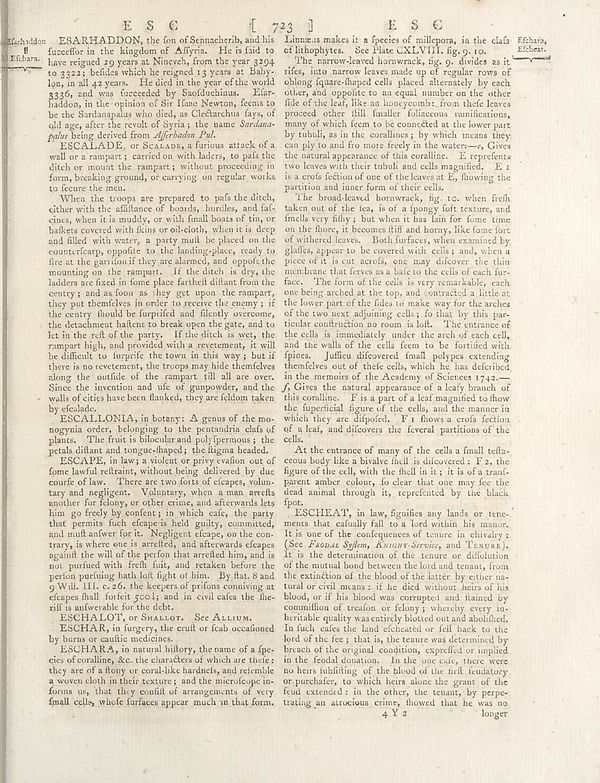
\includegraphics[width=0.85\textwidth]{../scans/page-1473-b3b602ef6a3d.jpg}
\caption*{Source scan: \texttt{page-1473-b3b602ef6a3d.jpg}}
\end{figure}

\end{document}
